\label{chapter:basic_latex}

% Paragraph descriping what the chapter is about
\blindtext

\section{A section with a definition and a theorem}
\label{sec:a_section_with_a_definition_and_a_theorem}

The above is a section. Here's a definition.

\begin{definition}[Conditional probability]
	\label{def:conditional_probability}
	The conditional probability of $A$ given $B$ is defined as
	\begin{equation*}
		P(A | B) = \frac{P(A \cap B)}{P(B)},
	\end{equation*}
	where $A \cap B$ denotes the intersection of $A$ and $B$.
\end{definition}

\begin{theorem}[Bayes theorem]
	Given $P(A | B)$, $P(A)$ and $P(B)$, we can compute $P(B | A)$ using 
	\begin{equation}
	\label{eqn:bayes_theorem}
	P(B | A) = \frac{P(A | B) P(B)}{P(A)}.
	\end{equation}
\end{theorem}
\begin{proof}
	Write $P(A \cap B)$ in two ways using the Definition \ref{def:conditional_probability} of conditional probability as follows.
	\begin{equation*}
		P(A \cap B) = P(A | B) P(B) \qquad P(B \cap A) = P(B | A) P(A)
	\end{equation*}
	The intersection is symmetric, meaning that $B \cap A = B \cap A$.
	Thus we can compare terms and write $P(A | B) P(B) = P(B | A) P(A)$, rearranging this gives Bayes theorem.
\end{proof}

Bayes theorem has many applications, such as the \emph{Naive Bayes Classifier}, which is a machine learning algorithm.
The classifier assigns a label to a piece of data, e.g. classifying an email as spam or not.
It's called ``naive'' since it assumes conditional independence.
Equation \eqref{eqn:bayes_theorem} has extensions when more variables are used.

\section{A section with an example}
In Section \ref{sec:a_section_with_a_definition_and_a_theorem} we gave a theorem, here's an example with a real world application.

\begin{example}[An example with numbers]
	Here's a little example with some numbers.
	\begin{align*}
		P(B | A) &= \frac{P(A | B) P(B)}{P(A)} \\
			 	 &= \frac{(0.3) (0.4)}{0.24} = \frac{0.12}{0.24} = \frac{1}{2}
	\end{align*}
	As you see, applications are everywhere.
\end{example}

\blindtext

\section{A section with a figure}
\blindtext
	\begin{figure}[ht!]
	\centering
	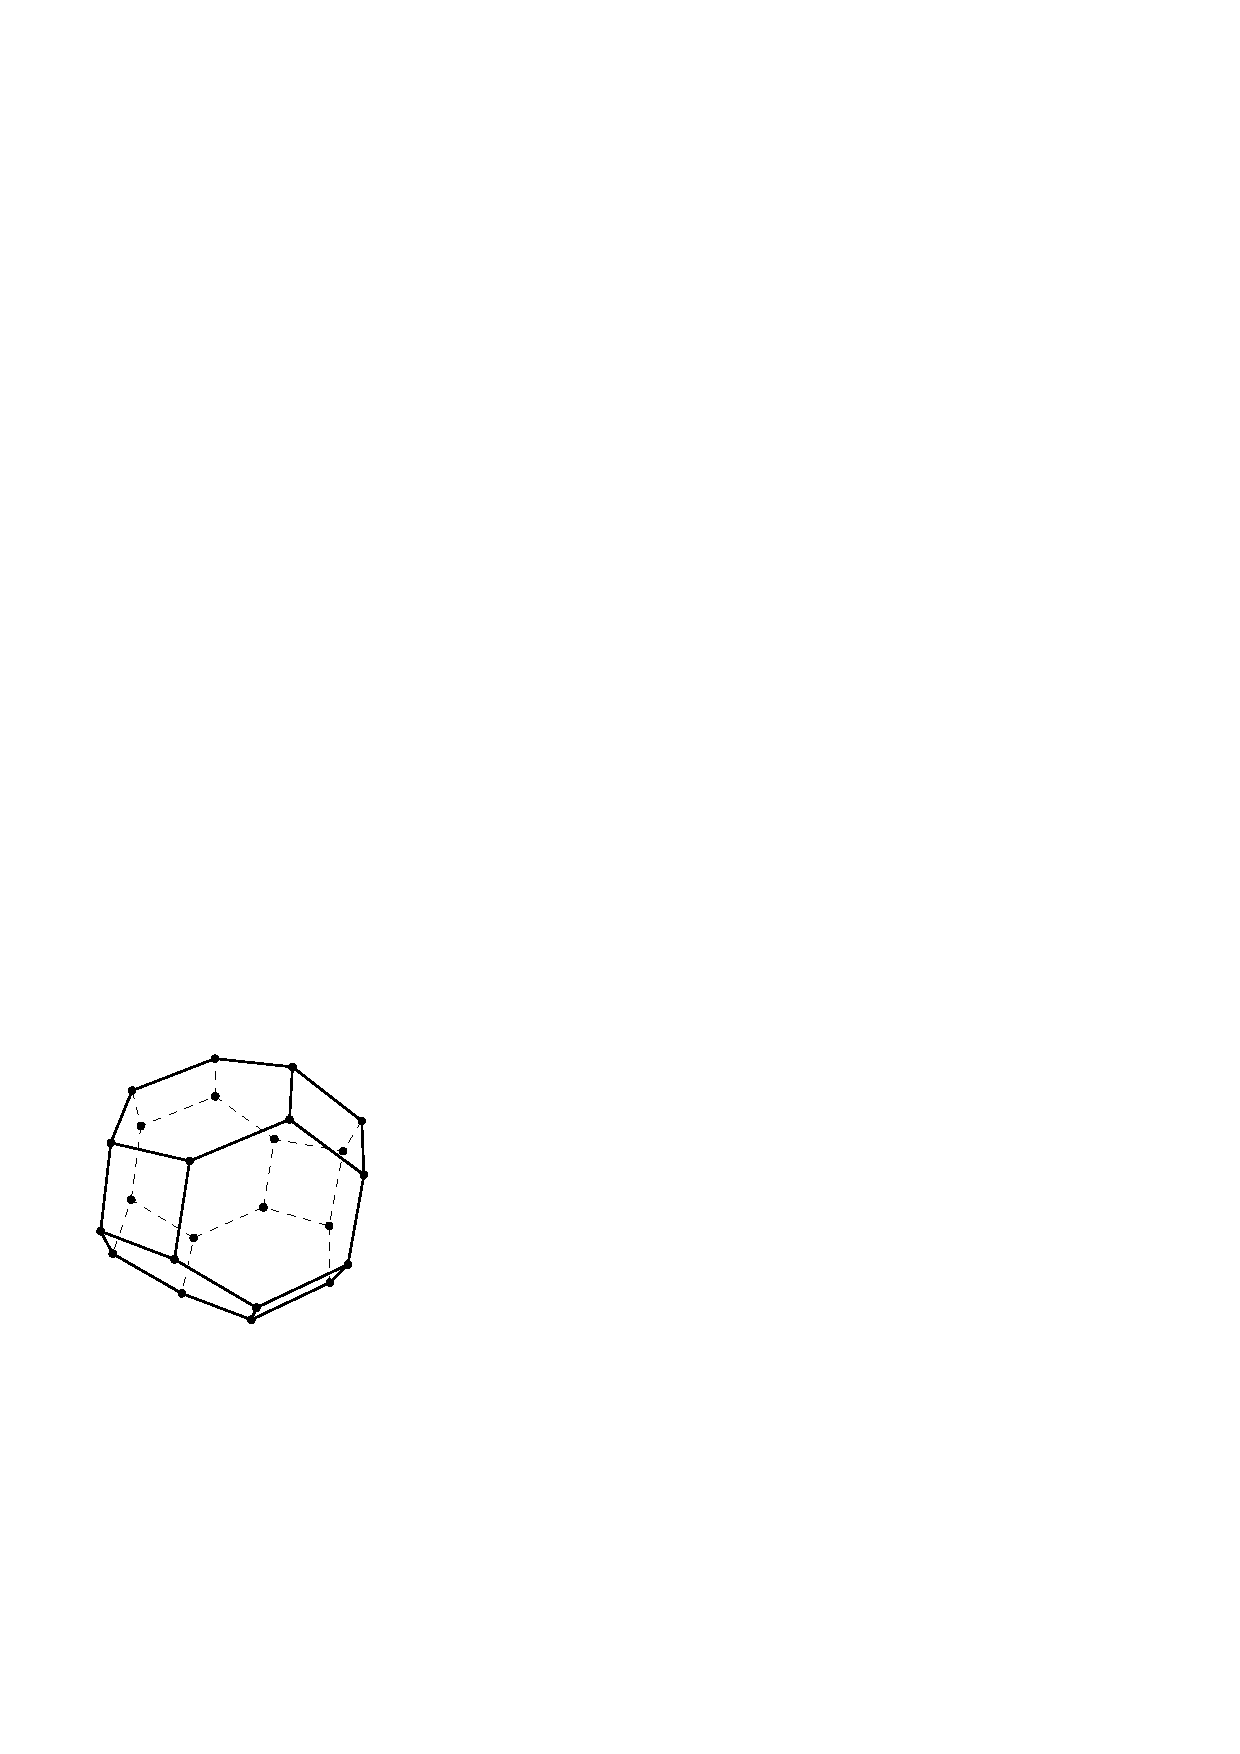
\includegraphics[width=0.3\linewidth]{figs/truncatedoctahedron}
	\caption{A pretty figure.}
	\label{fig:truncatedoctahedron}
	\end{figure}
\blindtext


